\chapter{Sistema de vinculación de componentes}\label{ch:sistema-de-vinculacion-de-componentes}

\note{Óscar: ¿no tendría sentido fundir este capítulo con el 4?}
  
En este capítulo se abordará la creación de un sistema de
vinculación de componentes para \textit{JAMS}, empezando por
la estructura de un componente y terminando por la carga
del mismo dentro de \textit{JAMS}.

\section{Estructura de un componente}\label{sec:estructura-de-un-componente}

Los componentes, al igual que en muchas aplicaciones \textit{Java},
están conformados por un archivo \textit{jar} con el código que
se desea usar en la aplicación principal.
Más concretamente, un componente de \textit{JAMS} debe contener
dos elementos esenciales:
\begin{itemize}
    \item \textbf{Punto de entrada}: está conformado por una
    clase que extiende a $Plugin$, una clase proporcionada por
    \textit{JAMS} que representa un componente.
    \textit{JAMS} crea una instancia de esta clase para
    poder ejecutar el código externo.
    \item \textbf{Archivo de metadatos}: confirmado por un archivo
    \textit{JSON}\cite{JSON} $plugin.json$ en la raíz del archivo \textit{jar}.
    Este archivo contiene los parámetros globales del componente,
    como pueden ser el \textbf{nombre}, la dirección del
    \textbf{punto de entrada}, la versión, los autores,
    o la descripción.
    Un ejemplo de archivo $plugin.json$ se puede observar en la
    figura \ref{fig:plugin-json}.
\end{itemize}


\begin{figure}[h]
    \centering
    \begin{lstlisting}[frame=single,label={lst:plugin-json}]
{
  "name": "NES4JAMS",
  "main": "io.github.gaeqs.nes4jams.NES4JAMS",
  "version": "0.1-ALPHA",
  "authors": [
    "Gael Rial Costas"
  ],
  "favicon": "/gui/icon/favicon.png",
  "description_node": "NES4JAMS_DESCRIPTION"
}
    \end{lstlisting}
    \caption{Ejemplo de archivo $plugin.json$}
    \label{fig:plugin-json}
\end{figure}

\subsection{Dependencias}\label{subsec:dependencias}

Un componente puede depender de otro componente.
Para realizar una inicialización correcta de los componentes
se proporcionan los parámetros $dependencies$
y $soft\_dependencies$, los cuales pueden utilizarse en
el archivo $plugin.json$.
Todos los componentes cuyo nombre esté dentro de una de estas
listas serán inicializados con anterioridad.
Si no se encuentra ningún componente que tenga el nombre
de algún valor de $dependencies$, el componente no
se inicializará, lanzando una excepción.
Cabe destacar que dos componentes no pueden conformar
una \textbf{dependencia cíclica}.

\subsection{Puntos de entrada}\label{subsec:puntos-de-entrada}

Como ya se ha mencionado, un punto de entrada está conformado
por una \textbf{clase que extiende a $Plugin$}.
El desarrollador puede extender dos métodos definidos por esta clase:
$onEnable$ y $onDisable$, que serán llamados cuando el
componente se vincula o desvincula de la aplicación principal.
Un ejemplo de punto de entrada se puede observar en la figura \ref{fig:entry-point}.

\begin{figure}[h]
    \centering
    \begin{lstlisting}[frame=single,label={lst:entry-point},language=Kotlin]
class MyPlugin : Plugin() {

    override fun onEnable() {
        println("My plugin has been enabled!")
        if (JamsApplication.isLoaded()) {
            loadApplicationData()
        }
    }

    override fun onDisable() {
        println("My plugin has been disabled!")
    }

    @Listener
    fun onApplicationLoad(event: JAMSApplicationPostInitEvent)
        = loadApplicationData()

    private fun loadApplicationData() {
        println("Now I can access the JavaFX application!")
    }

}
    \end{lstlisting}
    \caption{Ejemplo de punto de entrada de un componente desarrollado en \textit{Kotlin}}
    \label{fig:entry-point}
\end{figure}

El punto de entrada puede ser inicializado en diferentes
etapas del proyecto: el componente se cargará antes que el contexto
de \textit{JavaFX} si este ya estaba instalado en la aplicación
cuando esta se lanza.
El desarrollador debe \textbf{comprobar si el contexto se ha creado}
antes de añadir o modificar nuevos elementos.
Si el contexto aún no se ha creado, los componentes podrán
usar el evento $JAMSApplicationPostInitEvent$ para ejecutar
código cuando este se inicialice.
Este sistema de eventos se analizará en profundidad más adelante en esta memoria.


\section{Vinculación de un componente}\label{sec:vinculacion-de-un-componente}

Es posible vincular un componente de dos maneras diferentes:
cuando el usuario \textbf{instala el componente} desde la aplicación
y cuando \textbf{se inicializa la aplicación principal} y el componente
está ya instalado.
La vinculación de componentes difiere en varios aspectos en estas
dos situaciones: cuando se instala el componente, \textit{JAMS}
comprueba si \textbf{todas sus dependencias fuertes están presentes}.
Si esto no se cumple, el componente no se instala.
Cuando arranca aplicación principal debe vincular
una cantidad no definida de componentes, y por ello tiene que
generar un \textbf{grafo de dependencias} antes de inicializarlos.

\section{Desvinculación de un componente}\label{sec:desvinculacion-de-un-componente}

Un componente se desvincula de la aplicación principal
cuando \textbf{el usuario lo desinstala} desde
la configuración o cuando la \textbf{aplicación principal se cierra}.
De la misma manera que en la vinculación, el proceso de
desvinculación \textbf{difiere} en ambas circunstancias.
Para que un componente sea desinstalado, el usuario
debe desinstalar previamente \textbf{todos los componentes
que dependen} del componente desinstalado.
Se puede desinstalar el componente cuando no hay
ningún componente dependiente instalado.
Cuando la aplicación principal se cierra
\textbf{no se desvincula ningún componente},
si no que se llama únicamente a sus métodos $onDisable$, dejando
el proceso de desvinculación a la \textit{JVM}.

\section{Interfaz de usuario}\label{sec:interfaz-de-usuario}

Los usuarios pueden instalar o desinstalar componentes
desde la \textbf{ventana de configuración}, mostrada en la figura \ref{fig:plugin-ui}.
En esta interfaz se mostrará la lista de componentes
que están instalados junto con su nombre, su versión
y su descripción.

\begin{figure}[h]
    \centering
    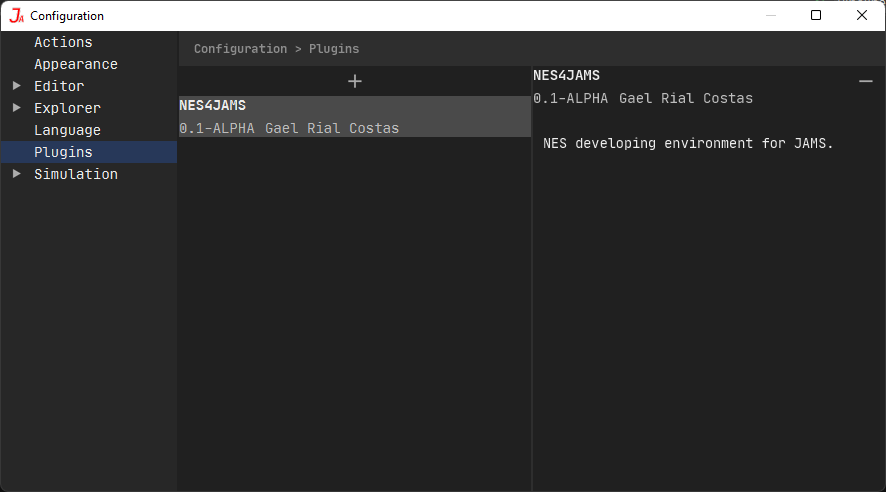
\includegraphics[width=\textwidth]{images/componentes/plugin-ui}
    \caption{Sección de componentes en la configuración}
    \label{fig:plugin-ui}
\end{figure}